% Created 2026-07-13 Mon 09:56
% Intended LaTeX compiler: pdflatex
\documentclass[11pt]{article}
\usepackage[utf8]{inputenc}
\usepackage[T1]{fontenc}
\usepackage{graphicx}
\usepackage{longtable}
\usepackage{wrapfig}
\usepackage{rotating}
\usepackage[normalem]{ulem}
\usepackage{amsmath}
\usepackage{amssymb}
\usepackage{capt-of}
\usepackage{hyperref}
\author{Auz Juan, Lanchimba Danny, Palomeque Matías, Quillupangui Ana María}
\date{2026-07-13}
\title{Análisis de Datos de Seguridad INEC 2025-2026}
\hypersetup{
 pdfauthor={Auz Juan, Lanchimba Danny, Palomeque Matías, Quillupangui Ana María},
 pdftitle={Análisis de Datos de Seguridad INEC 2025-2026},
 pdfkeywords={},
 pdfsubject={},
 pdfcreator={Emacs 27.1 (Org mode 9.7.5)}, 
 pdflang={Spanish}}
\begin{document}

\maketitle
\tableofcontents


\section{Análisis de Datos de Seguridad INEC}
\label{sec:orgf050cd8}

Este proyecto corresponde al trabajo final de semestre de la asignatura
\textbf{\textbf{Arquitectura de Computadores}}.

El objetivo es realizar un análisis de información estadística obtenida
desde los datos proporcionados por el Instituto Nacional de Estadística
y Censos (INEC), aplicando herramientas computacionales para la
extracción, procesamiento, análisis y visualización de datos.

\section{Formulación del problema}
\label{sec:orgb5669be}

Se desea realizar un análisis estadístico utilizando información
proporcionada por el INEC relacionada con seguridad.

Para esto, se utiliza un conjunto de datos en formato Excel (.xlsx) que contiene
información recopilada durante el año 2025 hasta febrero del 2026.

El objetivo es procesar los datos obtenidos, identificar patrones
relevantes y representar los resultados mediante tablas y gráficos
estadísticos utilizando Python.


\section{Descripción del código}
\label{sec:org1e6bbed}

En esta sección se detallan los componentes principales del código
desarrollado y la estrategia utilizada para resolver el problema.


\subsection{Librerías utilizadas y carga inicial de datos}
\label{sec:orgf410425}

Durante el procesamiento de la información se utilizan las siguientes
librerías:

\begin{itemize}
\item pandas
\item numpy
\item matplotlib
\item seaborn
\end{itemize}

En esta etapa se carga la hoja del archivo Excel que contiene la información
de femicidios por provincia proporcionada por el INEC.

\begin{verbatim}

import pandas as pd
import numpy as np
import matplotlib.pyplot as plt

archivo = "../../Datos de Seguridad Ecuador.xlsx"

df = pd.read_excel(
    archivo,
    sheet_name="3.femicidios_prov",
    header=3
)

# Eliminar columna vacía generada por el formato del Excel
df = df.drop(columns=df.columns[0])

\end{verbatim}
\section{Exploración inicial de los datos}
\label{sec:org2cf2bbb}

Antes de realizar el análisis se revisa la estructura del conjunto de datos para
identificar sus variables y características principales.
\begin{verbatim}

print("Dimensiones del conjunto de datos:")
print(df.shape)

print("\nPrimeras filas del conjunto de datos:")
print(df.head())

\end{verbatim}
\begin{verbatim}
Dimensiones del conjunto de datos:
(25, 147)

Primeras filas del conjunto de datos:
  Provincia de ocurrencia  2014-01-01 00:00:00  2014-02-01 00:00:00  2014-03-01 00:00:00  ...  2025-11-01 00:00:00  2025-12-01 00:00:00  2026-01-01 00:00:00  2026-02-01 00:00:00
0                   Azuay                    0                    0                    0  ...                    0                    0                    0                    0
1                 Bolívar                    0                    0                    0  ...                    0                    0                    0                    0
2                   Cañar                    0                    0                    0  ...                    0                    1                    0                    0
3                  Carchi                    0                    0                    0  ...                    0                    0                    0                    0
4                Cotopaxi                    0                    0                    0  ...                    0                    1                    0                    0

[5 rows x 147 columns]
\end{verbatim}


\subsection{Selección del periodo de análisis}
\label{sec:org2f6bbba}

Debido a que el archivo contiene información desde el año 2014 hasta
2026, se seleccionan únicamente los datos correspondientes al periodo
enero 2025- febrero 2026 para el análisis.

\begin{verbatim}

# Seleccionar columnas correspondientes a los años 2025 y 2026
columnas_periodo = [
    columna for columna in df.columns
    if "2025" in str(columna) or "2026" in str(columna)
]

# Crear nuevo DataFrame con provincias y periodo seleccionado
df_2025_2026 = df[["Provincia de ocurrencia"] + columnas_periodo]

print("Dimensiones del periodo seleccionado:")
print(df_2025_2026.shape)

print("\nColumnas seleccionadas:")
print(df_2025_2026.columns)

\end{verbatim}

\begin{verbatim}
Dimensiones del periodo seleccionado:
(25, 15)

Columnas seleccionadas:
Index(['Provincia de ocurrencia',       2025-01-01 00:00:00,
             2025-02-01 00:00:00,       2025-03-01 00:00:00,
             2025-04-01 00:00:00,       2025-05-01 00:00:00,
             2025-06-01 00:00:00,       2025-07-01 00:00:00,
             2025-08-01 00:00:00,       2025-09-01 00:00:00,
             2025-10-01 00:00:00,       2025-11-01 00:00:00,
             2025-12-01 00:00:00,       2026-01-01 00:00:00,
             2026-02-01 00:00:00],
      dtype='object')
\end{verbatim}



\section{Procesamiento de datos}
\label{sec:org489b36a}

En esta etapa se realizan las transformaciones necesarias para preparar
la información:

\begin{itemize}
\item Selección del periodo de análisis.
\item Verificación de valores faltantes.
\item Transformación del formato de los datos.
\item Preparación de la información para el análisis estadístico.
\end{itemize}

\begin{verbatim}

print(df_2025_2026.head())

\end{verbatim}
\begin{verbatim}
  Provincia de ocurrencia  2025-01-01 00:00:00  2025-02-01 00:00:00  2025-03-01 00:00:00  ...  2025-11-01 00:00:00  2025-12-01 00:00:00  2026-01-01 00:00:00  2026-02-01 00:00:00
0                   Azuay                    0                    1                    0  ...                    0                    0                    0                    0
1                 Bolívar                    0                    0                    0  ...                    0                    0                    0                    0
2                   Cañar                    0                    0                    0  ...                    0                    1                    0                    0
3                  Carchi                    0                    0                    0  ...                    0                    0                    0                    0
4                Cotopaxi                    0                    0                    0  ...                    0                    1                    0                    0

[5 rows x 15 columns]
\end{verbatim}


\subsection{Tratamiento de valores faltantes}
\label{sec:org3a19b41}

Se revisa la existencia de valores faltantes dentro del conjunto de datos
seleccionado.

\begin{verbatim}

print(df_2025_2026.isnull().sum().sum())

\end{verbatim}

\begin{verbatim}
0
\end{verbatim}

\subsection{Transformación de datos}
\label{sec:org65d7d35}

La información obtenida desde el Excel se encuentra en formato ancho,
donde cada mes corresponde a una columna. Para facilitar el análisis y
la generación de gráficos se transforma a un formato donde cada fila
representa una observación mensual.

\begin{verbatim}

# Transformación de formato ancho a formato largo

df_largo = df_2025_2026.melt(
    id_vars=["Provincia de ocurrencia"],
    var_name="Fecha",
    value_name="Femicidios"
)

# Convertir la columna fecha a formato fecha
df_largo["Fecha"] = pd.to_datetime(df_largo["Fecha"])

print("Dimensiones del nuevo conjunto de datos:")
print(df_largo.shape)

print("\nPrimeras filas:")
print(df_largo.head())

\end{verbatim}

\begin{verbatim}
Dimensiones del nuevo conjunto de datos:
(350, 3)

Primeras filas:
  Provincia de ocurrencia      Fecha  Femicidios
0                   Azuay 2025-01-01           0
1                 Bolívar 2025-01-01           0
2                   Cañar 2025-01-01           0
3                  Carchi 2025-01-01           0
4                Cotopaxi 2025-01-01           0
\end{verbatim}



\section{Análisis estadístico}
\label{sec:org5e3b193}

El análisis se realiza utilizando el conjunto de datos transformado
(df\textsubscript{largo}), donde cada fila representa el número de femicidios registrado
para una provincia en un mes determinado.

\subsection{Eliminación de registros agregados}
\label{sec:org424edd9}

El conjunto de datos contiene un registro correspondiente al Total Nacional,
el cual representa la suma de todas las provincias. Debido a que el análisis
se realizará a nivel provincial, este registro es eliminado para evitar
distorsionar los resultados estadísticos.

\begin{verbatim}

df_largo = df_largo[
    df_largo["Provincia de ocurrencia"] != "Total Nacional"
]

print("Número de provincias analizadas:")
print(df_largo["Provincia de ocurrencia"].nunique())

\end{verbatim}

\begin{verbatim}
Número de provincias analizadas:
24
\end{verbatim}

\subsection{Estadísticas descriptivas}
\label{sec:org0a8b7f1}

Se calculan medidas estadísticas descriptivas para conocer la distribución
general de los casos registrados.

\begin{verbatim}

estadisticos = (
    df_largo["Femicidios"]
    .describe()
    .reset_index()
)

estadisticos.columns = ["Medida", "Valor"]

table = [list(estadisticos.columns)] + [None] + estadisticos.values.tolist()

table

\end{verbatim}
\begin{center}
\begin{tabular}{lr}
Medida & Valor\\[0pt]
\hline
count & 336.0\\[0pt]
mean & 0.19047619047619047\\[0pt]
std & 0.46938996233925495\\[0pt]
min & 0.0\\[0pt]
25\% & 0.0\\[0pt]
50\% & 0.0\\[0pt]
75\% & 0.0\\[0pt]
max & 3.0\\[0pt]
\end{tabular}
\end{center}

\subsection{Total de femicidios por provincia}
\label{sec:org5d102ba}

Para identificar las provincias con mayor cantidad de casos durante el
periodo analizado se realiza una agrupación por provincia.

\begin{verbatim}

femicidios_provincia = (
    df_largo.groupby("Provincia de ocurrencia")["Femicidios"]
    .sum()
    .sort_values(ascending=False)
)

print(femicidios_provincia)

\end{verbatim}

\begin{verbatim}
Provincia de ocurrencia
Pichincha                         15
Guayas                             9
Esmeraldas                         7
Los Ríos                           6
Manabí                             3
Azuay                              3
Cotopaxi                           3
El Oro                             3
Tungurahua                         3
Imbabura                           3
Orellana                           2
Pastaza                            2
Santo Domingo de los Tsáchilas     2
Sucumbíos                          1
Zamora Chinchipe                   1
Cañar                              1
Chimborazo                         0
Carchi                             0
Bolívar                            0
Loja                               0
Napo                               0
Morona Santiago                    0
Galápagos                          0
Santa Elena                        0
Name: Femicidios, dtype: int64
\end{verbatim}


\subsection{Estadísticos por provincia}
\label{sec:org9ea8dc3}

A partir del total de femicidios registrados por provincia se calculan
medidas descriptivas para resumir el comportamiento de los datos.

\begin{verbatim}

estadisticos_provincia = (
    femicidios_provincia
    .describe()
    .reset_index()
)

estadisticos_provincia.columns = ["Medida", "Valor"]

table = [list(estadisticos_provincia)] + [None] + estadisticos_provincia.values.tolist()

table

\end{verbatim}

\begin{center}
\begin{tabular}{lr}
Medida & Valor\\[0pt]
\hline
count & 24.0\\[0pt]
mean & 2.6666666666666665\\[0pt]
std & 3.546788708807946\\[0pt]
min & 0.0\\[0pt]
25\% & 0.0\\[0pt]
50\% & 2.0\\[0pt]
75\% & 3.0\\[0pt]
max & 15.0\\[0pt]
\end{tabular}
\end{center}


\subsection{Evolución mensual de femicidios}
\label{sec:org7c24b5e}

Se agrupan los datos por mes para observar el comportamiento temporal
durante el periodo seleccionado.


\begin{verbatim}

femicidios_mes = (
    df_largo.groupby("Fecha")["Femicidios"]
    .sum()
)

print(femicidios_mes)

\end{verbatim}

\begin{verbatim}
Fecha
2025-01-01    5
2025-02-01    5
2025-03-01    6
2025-04-01    5
2025-05-01    6
2025-06-01    5
2025-07-01    2
2025-08-01    7
2025-09-01    3
2025-10-01    5
2025-11-01    4
2025-12-01    4
2026-01-01    4
2026-02-01    3
Name: Femicidios, dtype: int64
\end{verbatim}

\subsection{Frecuencia de registros por cantidad de femicidios}
\label{sec:org6365328}

Se analiza la frecuencia de los valores registrados para observar la
distribución de los casos.

\begin{verbatim}

print(df_largo["Femicidios"].value_counts().sort_index())

\end{verbatim}

\begin{verbatim}
Femicidios
0    282
1     45
2      8
3      1
Name: count, dtype: int64
\end{verbatim}


\subsection{Preparación de datos para visualización}
\label{sec:orgd473785}

Se generan estructuras resumidas que serán utilizadas posteriormente
para la creación de gráficos estadísticos.

\begin{verbatim}

print("Datos preparados:")
print("Provincias analizadas:", len(femicidios_provincia))
print("Meses analizados:", len(femicidios_mes))

\end{verbatim}

\begin{verbatim}
Datos preparados:
Provincias analizadas: 24
Meses analizados: 14
\end{verbatim}

\section{Presentación de resultados}
\label{sec:org3967973}

En esta sección se presentan los principales resultados obtenidos
a partir del análisis estadístico realizado sobre los datos de
femicidios registrados por provincia durante el periodo 2025-2026.


\subsection{Muestra aleatoria de datos}
\label{sec:orgc0ca81a}

Se presenta una muestra aleatoria de los datos procesados
después de la transformación al formato largo.

\begin{verbatim}

tabla_muestra = df_largo.sample(10).copy()

tabla_muestra["Fecha"] = tabla_muestra["Fecha"].astype(str).str[:10]

table = [list(tabla_muestra)] + [None] + tabla_muestra.values.tolist()

table

\end{verbatim}

\begin{center}
\begin{tabular}{lrr}
Provincia de ocurrencia & Fecha & Femicidios\\[0pt]
\hline
Chimborazo & 2025-06-01 & 0\\[0pt]
Zamora Chinchipe & 2025-12-01 & 0\\[0pt]
Carchi & 2025-01-01 & 0\\[0pt]
Guayas & 2025-08-01 & 2\\[0pt]
Guayas & 2025-09-01 & 0\\[0pt]
Manabí & 2025-09-01 & 0\\[0pt]
Esmeraldas & 2026-01-01 & 0\\[0pt]
Esmeraldas & 2025-12-01 & 0\\[0pt]
Santa Elena & 2025-07-01 & 0\\[0pt]
Bolívar & 2025-01-01 & 0\\[0pt]
\end{tabular}
\end{center}

**Provincias con mayor cantidad de femicidios registrados 

\begin{verbatim}

tabla_provincias = (
    femicidios_provincia
    .head(10)
    .reset_index()
)

table = [list(tabla_provincias)] + [None] + tabla_provincias.values.tolist()

table

\end{verbatim}

\begin{center}
\begin{tabular}{lr}
Provincia de ocurrencia & Femicidios\\[0pt]
\hline
Pichincha & 15\\[0pt]
Guayas & 9\\[0pt]
Esmeraldas & 7\\[0pt]
Los Ríos & 6\\[0pt]
Manabí & 3\\[0pt]
Azuay & 3\\[0pt]
Cotopaxi & 3\\[0pt]
El Oro & 3\\[0pt]
Tungurahua & 3\\[0pt]
Imbabura & 3\\[0pt]
\end{tabular}
\end{center}

\subsection{Femicidios acumulados por provincia}
\label{sec:org873a22c}

La siguiente gráfica permite observar la distribución de los casos
acumulados de femicidio por provincia durante el periodo analizado.

\begin{verbatim}

plt.figure(figsize=(10,6))

femicidios_provincia.plot(kind="bar")

plt.title("Femicidios acumulados por provincia (2025-2026)")
plt.xlabel("Provincia")
plt.ylabel("Número de femicidios")

plt.xticks(rotation=90)

plt.tight_layout()

archivo="./images/femicidios_provincia.png"

plt.savefig(archivo)

plt.close()

archivo

\end{verbatim}

\begin{center}
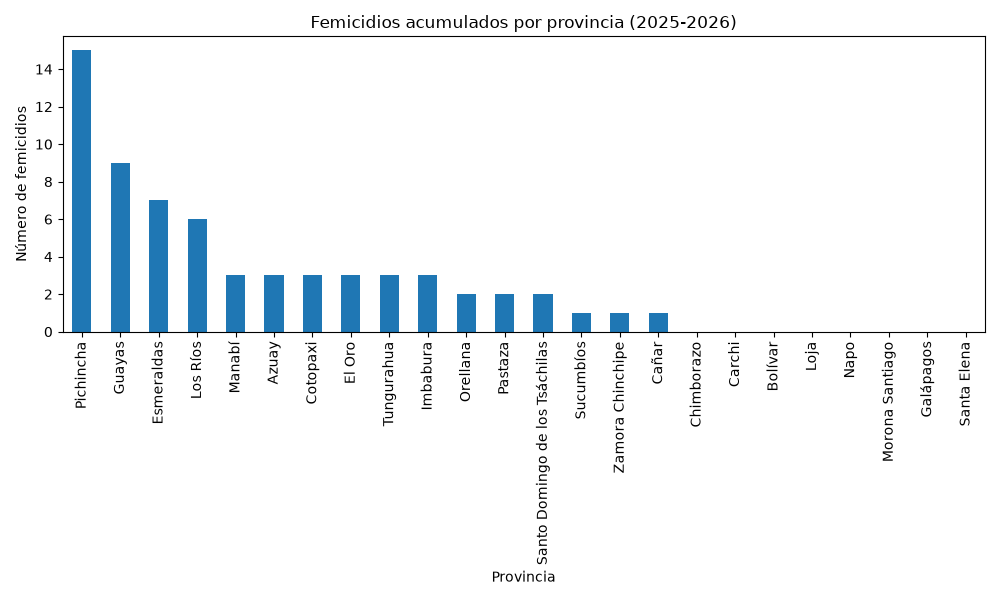
\includegraphics[width=.9\linewidth]{./images/femicidios_provincia.png}
\end{center}


\subsection{Evolución mensual de femicidios}
\label{sec:org0de9a40}

La siguiente gráfica muestra la variación mensual de los casos registrados
durante el periodo seleccionado.


\begin{verbatim}

plt.figure(figsize=(12,5))

plt.plot(
    femicidios_mes.index,
    femicidios_mes.values,
    marker="o"
)

plt.title("Evolución mensual de femicidios (2025-2026)")
plt.xlabel("Mes")
plt.ylabel("Número de femicidios")

# Mostrar todos los meses
plt.xticks(
    femicidios_mes.index,
    [fecha.strftime("%b-%Y") for fecha in femicidios_mes.index],
    rotation=45
)

plt.grid()

plt.tight_layout()

archivo="./images/evolucion_mensual_femicidios.png"

plt.savefig(archivo)

plt.close()

archivo

\end{verbatim}

\begin{center}
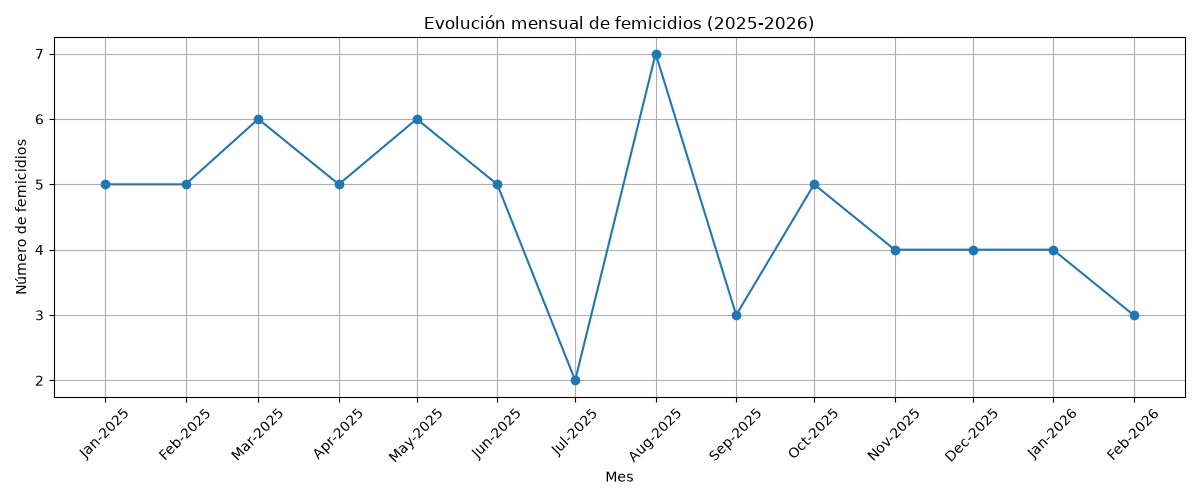
\includegraphics[width=.9\linewidth]{./images/evolucion_mensual_femicidios.png}
\end{center}


\subsection{Frecuencia de registros según cantidad de femicidios}
\label{sec:org09d0aa7}

La gráfica representa la frecuencia con la que aparecen diferentes
cantidades de femicidios en los registros mensuales por provincia.

\begin{verbatim}

frecuencia = df_largo["Femicidios"].value_counts().sort_index()

plt.figure(figsize=(7,5))

frecuencia.plot(kind="bar")

plt.title("Frecuencia de registros según cantidad de femicidios")
plt.xlabel("Cantidad de femicidios")
plt.ylabel("Número de registros")

plt.xticks(rotation=0)

plt.tight_layout()

archivo="./images/frecuencia_femicidios.png"

plt.savefig(archivo)

plt.close()

archivo

\end{verbatim}

\begin{center}
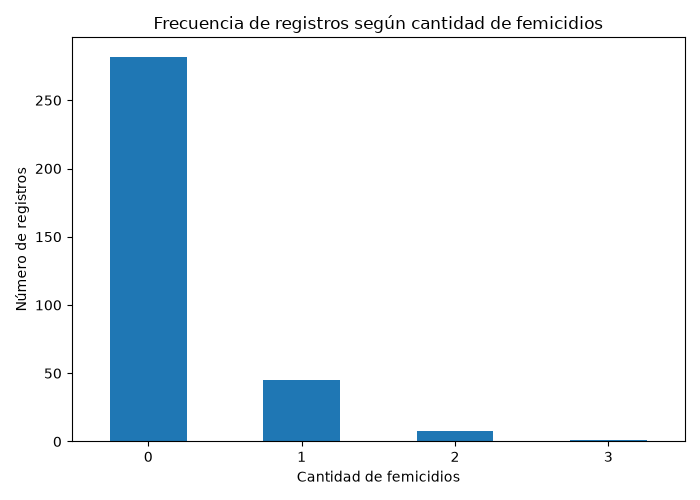
\includegraphics[width=.9\linewidth]{./images/frecuencia_femicidios.png}
\end{center}

\subsection{Interpretación de los datos}
\label{sec:orge55c5dd}
\begin{enumerate}
\item \textbf{\textbf{Interpretación de estadísticas descriptivas generales:}}
El análisis descriptivo realizado sobre los registros mensuales pro
provincia muestra que durante el periodo 2025-2026 se analizaron
336 observaciones, correspondientes a 24 provincias y 14 meses. El
promedio obtenido fue de 0.19 femicidios por provincia-mes, esto
indica que la ocurrencia de estos eventos dentro de una unidad
específica de análisis es baja.
La desviación estándar de 0.47 evidencia una dispersión reducida de
los datos alrededor del promedio. Además, los valores
correspondientes al primer, segundo y tercer cuartil son iguales a
cero, indicando que al menos el 75\% de los registros mensuales por
provincia no demuestran casos registrados.
El valor máximo observado fue de 3 femicidios en una provincia
durante un mes determinado, mostrando que, aunque la mayoría de
registros presentan valores bajos, existen periodos específicos con
concentraciones en mayores casos.
\item \textbf{\textbf{Interpretación por provincia:}}
Al analizar la distribución acumulada por provincia se observa que
los registros no se distribuyen uniformemente en el territorio
nacional. Pichincha concentra la mayor cantidad de casos con 15
registros, seguida de Guayas con 9 casos y Esmeraldas con 7.
La diferencia entre el valor máximo y el valor mínimo evidencia una
variabilidad importante entre provincias. Algunas provincias no
registraron casos durante el periodo analizado, mientras que otras
presentan una mayor concentración de eventos.
Los estadísticos calculados por provincia muestran una media de
2.67 casos y una mediana de 2 casos, lo que indica que la mitad de
las provincias presentan valores iguales o inferiores a dos
registros durante periodo.
\item \textbf{\textbf{Interpretación Temporal:}}
El análisis temporal permite observar la evolución mensual de los
femicidios registrados. Durante el periodo estudiado los valores
mensuales presentan fluctuaciones moderadas, sin una tendencia
creciente o decreciente claramente definida.
El mayor número de casos se registró en agosto de 2025 con 7
femicidios, mientras que julio presentó el menor valor con 2
casos. Estas variaciones muestran que la ocurrencia de estos
eventos presenta cambios entre meses, pero debido al tamaño del
periodo analizado no es posible establecer una tendencia histórica.
\item \textbf{\textbf{Interpretación de la frecuencia:}}
La distribución de la frecuencia evidencia que la mayoría de
observaciones corresponden a meses y provincias sin registros de
femicidio. De las 336 observaciones analizadas, 282 presentan un
valor de cero, mientras que únicamente 54 registros presentan uno o
más casos.
Este comportamiento explica por qué las medidas descriptivas
presentan valores bajos y demuestra que los femicidios corresponden
a eventos de baja frecuencia cuando se analizan individualmente por
provincia y mes
\item \textbf{\textbf{Conclusión General}}
En conjunto, el análisis estadístico permitió identificar varios
factores relevantes en los registros de femicidios del Ecuador
durante el periodo 2025-2026. Los resultados muestran una
concentración de casos en determinadas provincias, principalmente
Pichincha y Guayas, mientras que gran parte de las provincias
presentan valores reducidos o nulos.
El análisis descriptivo evidencia que la mayoría de registros
mensuales no presentan casos, por lo que las medidas como la media
y los cuartiles reflejan una distribución con alta presencia de
valores cero. Sin embargo, los valores máximos observados muestran
la existencia de periodos específicos con mayor concentración de
casos.
\end{enumerate}

\section{Referencias}
\label{sec:orgc483515}

\begin{itemize}
\item \href{https://orgmode.org/}{Org Mode Documentation}
\item \href{https://pandas.pydata.org/docs/}{Pandas Documentation}
\item \href{https://matplotlib.org/stable/}{Matplotlib Documentation}
\item \href{https://www.ecuadorencifras.gob.ec/}{Instituto Nacional de Estadística y Censos (INEC)}
\end{itemize}
\end{document}
